\begin{figure*}[t]
  \centering
  \subcaptionbox{\label{fig:interfaces-edit}Interface to evaluate language quality on CNN/Daily Mail}[0.47\linewidth]{%
    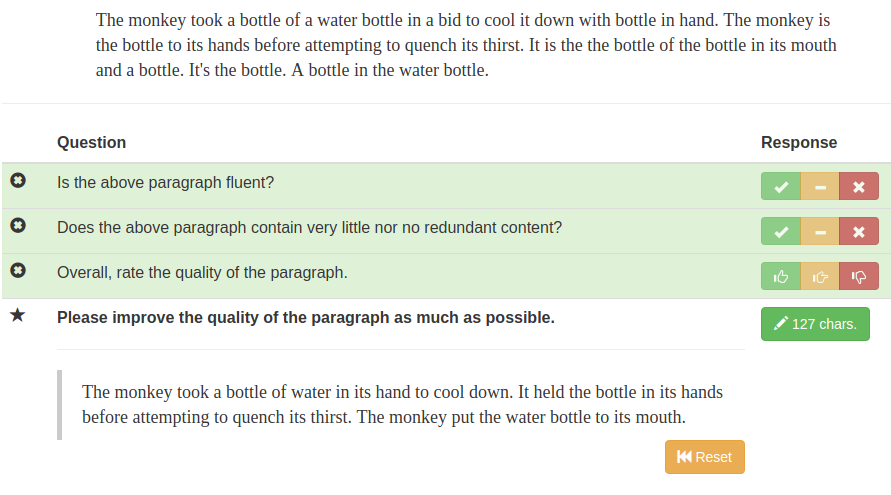
\includegraphics[width=0.47\textwidth]{figures/edit.png}
  }\hfill
  \subcaptionbox{\label{fig:interfaces-qa}Interface to judge answer correctness on MS MARCO}[0.47\linewidth]{%
    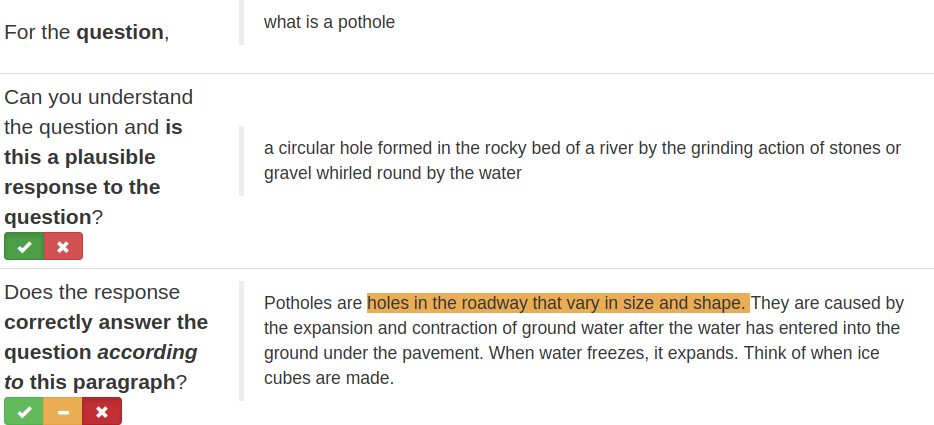
\includegraphics[width=0.47\textwidth]{figures/qa.png}
  }
  \caption{\label{fig:tasks} Screenshots of the annotation interfaces we used to measure (a) summary language quality on CNN/Daily Mail and (b) answer correctness on MS MARCO tasks.
  }
\end{figure*}

\begin{table}[t]
  \centering
  \begin{figure*}[t]
  \centering
  \subcaptionbox{\label{fig:interfaces-edit}Interface to evaluate language quality on CNN/Daily Mail}[0.47\linewidth]{%
    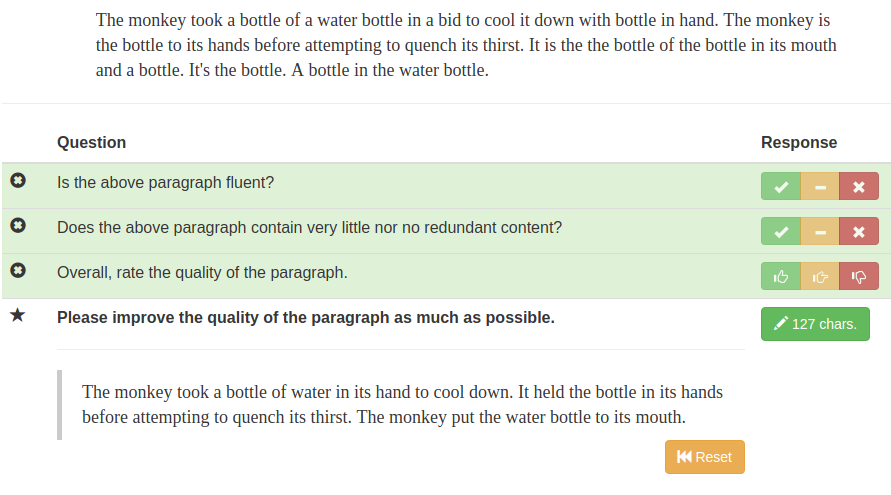
\includegraphics[width=0.47\textwidth]{figures/edit.png}
  }\hfill
  \subcaptionbox{\label{fig:interfaces-qa}Interface to judge answer correctness on MS MARCO}[0.47\linewidth]{%
    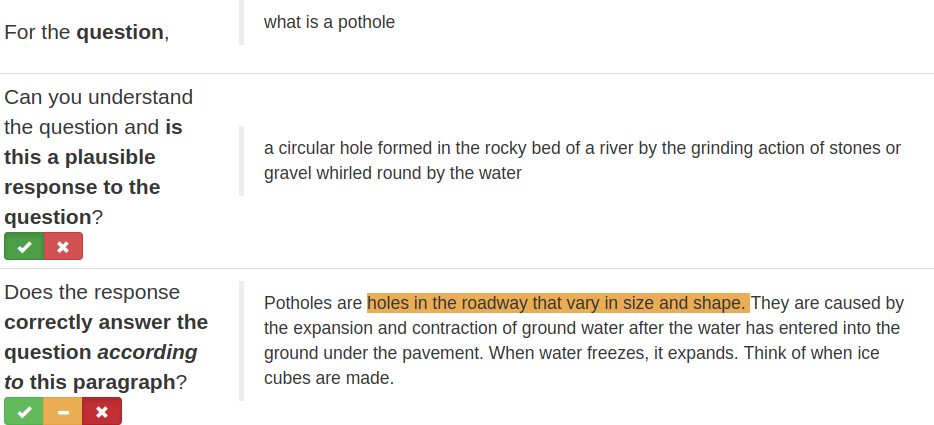
\includegraphics[width=0.47\textwidth]{figures/qa.png}
  }
  \caption{\label{fig:tasks} Screenshots of the annotation interfaces we used to measure (a) summary language quality on CNN/Daily Mail and (b) answer correctness on MS MARCO tasks.
  }
\end{figure*}

\begin{table}[t]
  \centering
  \begin{figure*}[t]
  \centering
  \subcaptionbox{\label{fig:interfaces-edit}Interface to evaluate language quality on CNN/Daily Mail}[0.47\linewidth]{%
    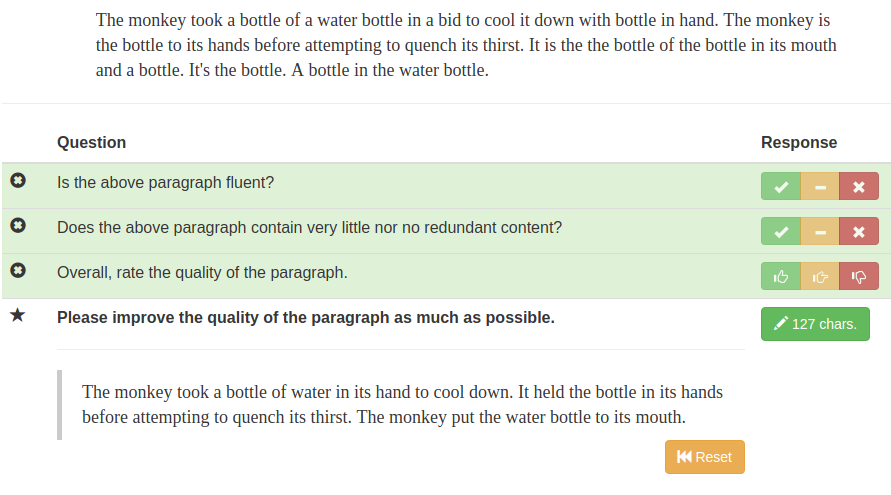
\includegraphics[width=0.47\textwidth]{figures/edit.png}
  }\hfill
  \subcaptionbox{\label{fig:interfaces-qa}Interface to judge answer correctness on MS MARCO}[0.47\linewidth]{%
    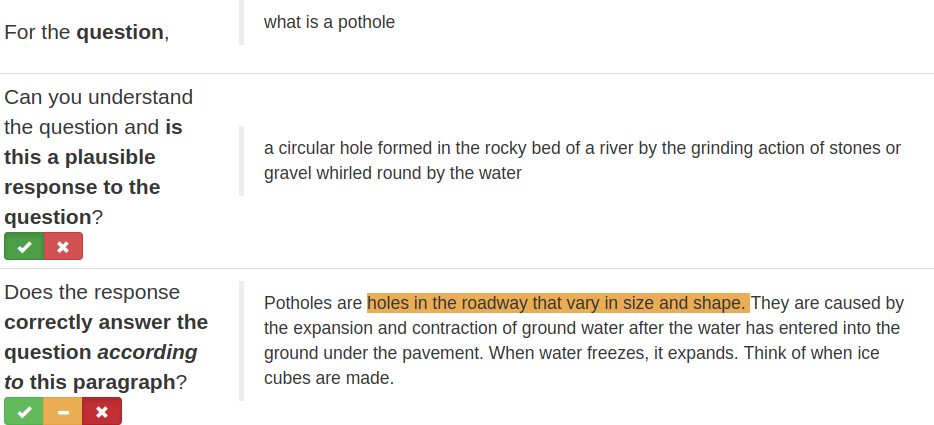
\includegraphics[width=0.47\textwidth]{figures/qa.png}
  }
  \caption{\label{fig:tasks} Screenshots of the annotation interfaces we used to measure (a) summary language quality on CNN/Daily Mail and (b) answer correctness on MS MARCO tasks.
  }
\end{figure*}

\begin{table}[t]
  \centering
  \begin{figure*}[t]
  \centering
  \subcaptionbox{\label{fig:interfaces-edit}Interface to evaluate language quality on CNN/Daily Mail}[0.47\linewidth]{%
    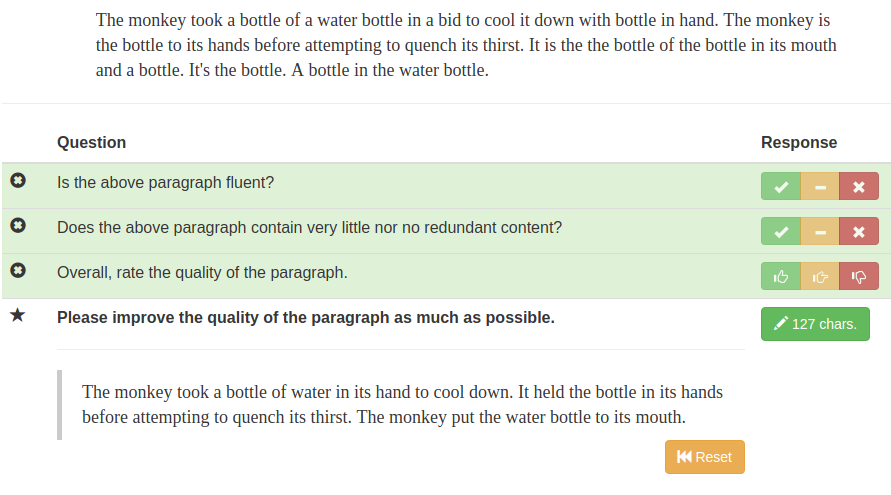
\includegraphics[width=0.47\textwidth]{figures/edit.png}
  }\hfill
  \subcaptionbox{\label{fig:interfaces-qa}Interface to judge answer correctness on MS MARCO}[0.47\linewidth]{%
    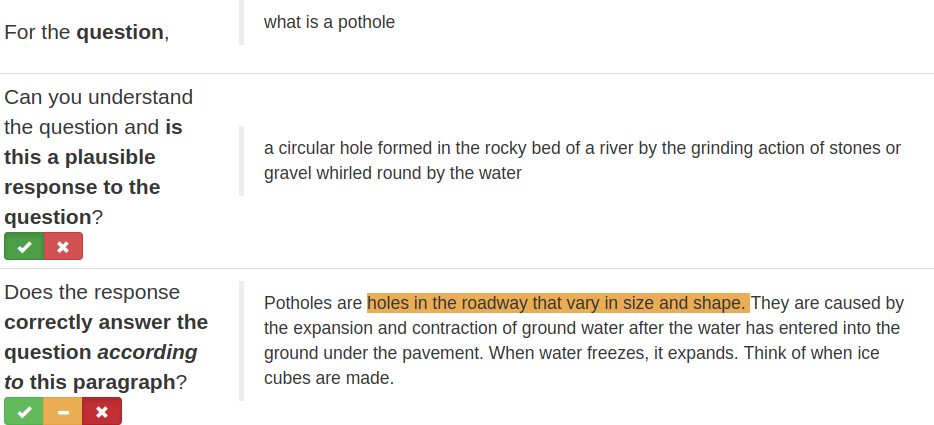
\includegraphics[width=0.47\textwidth]{figures/qa.png}
  }
  \caption{\label{fig:tasks} Screenshots of the annotation interfaces we used to measure (a) summary language quality on CNN/Daily Mail and (b) answer correctness on MS MARCO tasks.
  }
\end{figure*}

\begin{table}[t]
  \centering
  \input{tasks.table}
  \caption{\label{tab:dataset} A summary of the key statistics, human metric variance ($\sigma^2_f$) and annotator variance ($\sigma^2_a$) for different datasets, CNN/Daily Mail (CDM) and MS MARCO in our evaluation benchmark.
  We observe that the relative variance ($\gamma$) is fairly high for most evaluation prompts, upper bounding the data efficiency on these tasks.
  A notable exception is the \texttt{Edit} prompt wherein systems are compared on the number of post-edits required to improve their quality.
  }
\end{table}

\section{\label{sec:tasks} Tasks and datasets}

In order to compare different approaches to evaluating systems, we first collected human judgments for the output of several automatic summarization and open-response question answering systems using Amazon Mechanical Turk.
Details of instructions provided and quality assurance steps taken are provided in \refapp{interfaces} of the supplementary material.
In this section, we'll briefly describe how we collected this data.

\paragraph{Evaluating language quality in automatic summarization.}
In automatic summarization, systems must generate a short (on average two or three sentence) summary of an article: for our study, we chose articles from the CNN/Daily Mail (CDM) dataset~\citep{hermann2015read,nallapati2016abstractive} which come paired with reference summaries in the form of story highlights.
We focus on the \textit{language quality} of summaries and leave evaluating content selection to future work.

For each summary, we collected human judgments on a scale from 1--3 (\reffig{interfaces-edit}) for fluency, (lack of) redundancy, and overall quality of the summary using guidelines from the DUC summarization challenge~\citep{dang2006overview}.
As an alternate human metric, we also asked workers to post-edit the system's summary to improve its quality, similar to the post-editing step in MT evaluations~\citep{snover2006ter}.
Obtaining judgments costs about \$0.15 per summary and this cost rises to about \$0.40 per summary for post-editing.

We collected judgments on the summaries generated by the \texttt{seq2seq} and \texttt{pointer} models of \citet{see2017point}, the \texttt{ml} and \texttt{ml+rl} models of \citet{paulus2018deep}, and the reference summaries.\footnote{%
All system output was obtained from the original authors through private communication.} 
Before presenting the summaries to human annotators, we performed some minimal post-processing: we true-cased and de-tokenized the output of \texttt{seq2seq} and \texttt{pointer} using Stanford CoreNLP~\citep{manning2014stanford} and replaced ``unknown'' tokens in each system with a special symbol ($\blacksquare$).


\paragraph{Evaluating answer correctness.}
Next, we look at evaluating the correctness of system outputs in question answering using the MS MARCO question answering dataset~\citep{nguyen2016ms}.
Here, each system is provided with a question and up to 10 paragraphs of context.
The system generates open-response answers that do not need to be tied to a span in any paragraph.

We first ask annotators to judge if the output is even plausible for the question,
and if yes,
ask them identify if it is correct according to each context paragraph. 
We found that requiring annotators to highlight regions in the text that support their decision
substantially improved the quality of the output without increasing costs.
Annotations cost \$0.40 per system response.\footnote{%
  This cost could be significantly reduced if systems also specify which passage they used to generate the answer.
}

While our goal is to evaluate the correctness of the provided answer, we found that there are often answers which may be correct or incorrect depending on the context.
For example, the question ``what is a pothole'' is typically understood to refer to a hole in a roadway, but also refers to a geological feature (\reffig{interfaces-qa}).
This is reflected when annotators mark one context paragraph to support the given answer but mark another to contradict it.
We evaluated systems based on both the average correctness (AvgCorrect) of their answers across all paragraphs
as well as whether their answer is correct according to any paragraph (AnyCorrect).

We collected annotations on the systems generated by the \texttt{fastqa} and
\texttt{fastqa\_ext} from \citet{weissenborn2017fastqa} and the \texttt{snet} and \texttt{snet.ens}(emble) models from \citet{tan2018s}, along with reference answers.
The answers generated by the systems were used without any post-processing.
Surprisingly, we found that the correctness of the reference answers (according to the AnyCorrect metric) was only 73.5\%,
only 2\% above that of the leading system ($\texttt{snet.ens}$).
We manually inspected 30 reference answers which were annotated incorrectly and found that of those, 
about 95\% were indeed incorrect.
However, 62\% are actually answerable from some paragraph,
indicating that the real ceiling performance on this dataset is around 90\% and
that there is still room for improvement on this task.

  \caption{\label{tab:dataset} A summary of the key statistics, human metric variance ($\sigma^2_f$) and annotator variance ($\sigma^2_a$) for different datasets, CNN/Daily Mail (CDM) and MS MARCO in our evaluation benchmark.
  We observe that the relative variance ($\gamma$) is fairly high for most evaluation prompts, upper bounding the data efficiency on these tasks.
  A notable exception is the \texttt{Edit} prompt wherein systems are compared on the number of post-edits required to improve their quality.
  }
\end{table}

\section{\label{sec:tasks} Tasks and datasets}

In order to compare different approaches to evaluating systems, we first collected human judgments for the output of several automatic summarization and open-response question answering systems using Amazon Mechanical Turk.
Details of instructions provided and quality assurance steps taken are provided in \refapp{interfaces} of the supplementary material.
In this section, we'll briefly describe how we collected this data.

\paragraph{Evaluating language quality in automatic summarization.}
In automatic summarization, systems must generate a short (on average two or three sentence) summary of an article: for our study, we chose articles from the CNN/Daily Mail (CDM) dataset~\citep{hermann2015read,nallapati2016abstractive} which come paired with reference summaries in the form of story highlights.
We focus on the \textit{language quality} of summaries and leave evaluating content selection to future work.

For each summary, we collected human judgments on a scale from 1--3 (\reffig{interfaces-edit}) for fluency, (lack of) redundancy, and overall quality of the summary using guidelines from the DUC summarization challenge~\citep{dang2006overview}.
As an alternate human metric, we also asked workers to post-edit the system's summary to improve its quality, similar to the post-editing step in MT evaluations~\citep{snover2006ter}.
Obtaining judgments costs about \$0.15 per summary and this cost rises to about \$0.40 per summary for post-editing.

We collected judgments on the summaries generated by the \texttt{seq2seq} and \texttt{pointer} models of \citet{see2017point}, the \texttt{ml} and \texttt{ml+rl} models of \citet{paulus2018deep}, and the reference summaries.\footnote{%
All system output was obtained from the original authors through private communication.} 
Before presenting the summaries to human annotators, we performed some minimal post-processing: we true-cased and de-tokenized the output of \texttt{seq2seq} and \texttt{pointer} using Stanford CoreNLP~\citep{manning2014stanford} and replaced ``unknown'' tokens in each system with a special symbol ($\blacksquare$).


\paragraph{Evaluating answer correctness.}
Next, we look at evaluating the correctness of system outputs in question answering using the MS MARCO question answering dataset~\citep{nguyen2016ms}.
Here, each system is provided with a question and up to 10 paragraphs of context.
The system generates open-response answers that do not need to be tied to a span in any paragraph.

We first ask annotators to judge if the output is even plausible for the question,
and if yes,
ask them identify if it is correct according to each context paragraph. 
We found that requiring annotators to highlight regions in the text that support their decision
substantially improved the quality of the output without increasing costs.
Annotations cost \$0.40 per system response.\footnote{%
  This cost could be significantly reduced if systems also specify which passage they used to generate the answer.
}

While our goal is to evaluate the correctness of the provided answer, we found that there are often answers which may be correct or incorrect depending on the context.
For example, the question ``what is a pothole'' is typically understood to refer to a hole in a roadway, but also refers to a geological feature (\reffig{interfaces-qa}).
This is reflected when annotators mark one context paragraph to support the given answer but mark another to contradict it.
We evaluated systems based on both the average correctness (AvgCorrect) of their answers across all paragraphs
as well as whether their answer is correct according to any paragraph (AnyCorrect).

We collected annotations on the systems generated by the \texttt{fastqa} and
\texttt{fastqa\_ext} from \citet{weissenborn2017fastqa} and the \texttt{snet} and \texttt{snet.ens}(emble) models from \citet{tan2018s}, along with reference answers.
The answers generated by the systems were used without any post-processing.
Surprisingly, we found that the correctness of the reference answers (according to the AnyCorrect metric) was only 73.5\%,
only 2\% above that of the leading system ($\texttt{snet.ens}$).
We manually inspected 30 reference answers which were annotated incorrectly and found that of those, 
about 95\% were indeed incorrect.
However, 62\% are actually answerable from some paragraph,
indicating that the real ceiling performance on this dataset is around 90\% and
that there is still room for improvement on this task.

  \caption{\label{tab:dataset} A summary of the key statistics, human metric variance ($\sigma^2_f$) and annotator variance ($\sigma^2_a$) for different datasets, CNN/Daily Mail (CDM) and MS MARCO in our evaluation benchmark.
  We observe that the relative variance ($\gamma$) is fairly high for most evaluation prompts, upper bounding the data efficiency on these tasks.
  A notable exception is the \texttt{Edit} prompt wherein systems are compared on the number of post-edits required to improve their quality.
  }
\end{table}

\section{\label{sec:tasks} Tasks and datasets}

In order to compare different approaches to evaluating systems, we first collected human judgments for the output of several automatic summarization and open-response question answering systems using Amazon Mechanical Turk.
Details of instructions provided and quality assurance steps taken are provided in \refapp{interfaces} of the supplementary material.
In this section, we'll briefly describe how we collected this data.

\paragraph{Evaluating language quality in automatic summarization.}
In automatic summarization, systems must generate a short (on average two or three sentence) summary of an article: for our study, we chose articles from the CNN/Daily Mail (CDM) dataset~\citep{hermann2015read,nallapati2016abstractive} which come paired with reference summaries in the form of story highlights.
We focus on the \textit{language quality} of summaries and leave evaluating content selection to future work.

For each summary, we collected human judgments on a scale from 1--3 (\reffig{interfaces-edit}) for fluency, (lack of) redundancy, and overall quality of the summary using guidelines from the DUC summarization challenge~\citep{dang2006overview}.
As an alternate human metric, we also asked workers to post-edit the system's summary to improve its quality, similar to the post-editing step in MT evaluations~\citep{snover2006ter}.
Obtaining judgments costs about \$0.15 per summary and this cost rises to about \$0.40 per summary for post-editing.

We collected judgments on the summaries generated by the \texttt{seq2seq} and \texttt{pointer} models of \citet{see2017point}, the \texttt{ml} and \texttt{ml+rl} models of \citet{paulus2018deep}, and the reference summaries.\footnote{%
All system output was obtained from the original authors through private communication.} 
Before presenting the summaries to human annotators, we performed some minimal post-processing: we true-cased and de-tokenized the output of \texttt{seq2seq} and \texttt{pointer} using Stanford CoreNLP~\citep{manning2014stanford} and replaced ``unknown'' tokens in each system with a special symbol ($\blacksquare$).


\paragraph{Evaluating answer correctness.}
Next, we look at evaluating the correctness of system outputs in question answering using the MS MARCO question answering dataset~\citep{nguyen2016ms}.
Here, each system is provided with a question and up to 10 paragraphs of context.
The system generates open-response answers that do not need to be tied to a span in any paragraph.

We first ask annotators to judge if the output is even plausible for the question,
and if yes,
ask them identify if it is correct according to each context paragraph. 
We found that requiring annotators to highlight regions in the text that support their decision
substantially improved the quality of the output without increasing costs.
Annotations cost \$0.40 per system response.\footnote{%
  This cost could be significantly reduced if systems also specify which passage they used to generate the answer.
}

While our goal is to evaluate the correctness of the provided answer, we found that there are often answers which may be correct or incorrect depending on the context.
For example, the question ``what is a pothole'' is typically understood to refer to a hole in a roadway, but also refers to a geological feature (\reffig{interfaces-qa}).
This is reflected when annotators mark one context paragraph to support the given answer but mark another to contradict it.
We evaluated systems based on both the average correctness (AvgCorrect) of their answers across all paragraphs
as well as whether their answer is correct according to any paragraph (AnyCorrect).

We collected annotations on the systems generated by the \texttt{fastqa} and
\texttt{fastqa\_ext} from \citet{weissenborn2017fastqa} and the \texttt{snet} and \texttt{snet.ens}(emble) models from \citet{tan2018s}, along with reference answers.
The answers generated by the systems were used without any post-processing.
Surprisingly, we found that the correctness of the reference answers (according to the AnyCorrect metric) was only 73.5\%,
only 2\% above that of the leading system ($\texttt{snet.ens}$).
We manually inspected 30 reference answers which were annotated incorrectly and found that of those, 
about 95\% were indeed incorrect.
However, 62\% are actually answerable from some paragraph,
indicating that the real ceiling performance on this dataset is around 90\% and
that there is still room for improvement on this task.

  \caption{\label{tab:dataset} A summary of the key statistics, human metric variance ($\sigma^2_f$) and annotator variance ($\sigma^2_a$) for different datasets, CNN/Daily Mail (CDM) and MS MARCO in our evaluation benchmark.
  We observe that the relative variance ($\gamma$) is fairly high for most evaluation prompts, upper bounding the data efficiency on these tasks.
  A notable exception is the \texttt{Edit} prompt wherein systems are compared on the number of post-edits required to improve their quality.
  }
\end{table}

\section{\label{sec:tasks} Tasks and datasets}

In order to compare different approaches to evaluating systems, we first collected human judgments for the output of several automatic summarization and open-response question answering systems using Amazon Mechanical Turk.
Details of instructions provided and quality assurance steps taken are provided in \refapp{interfaces} of the supplementary material.
In this section, we'll briefly describe how we collected this data.

\paragraph{Evaluating language quality in automatic summarization.}
In automatic summarization, systems must generate a short (on average two or three sentence) summary of an article: for our study, we chose articles from the CNN/Daily Mail (CDM) dataset~\citep{hermann2015read,nallapati2016abstractive} which come paired with reference summaries in the form of story highlights.
We focus on the \textit{language quality} of summaries and leave evaluating content selection to future work.

For each summary, we collected human judgments on a scale from 1--3 (\reffig{interfaces-edit}) for fluency, (lack of) redundancy, and overall quality of the summary using guidelines from the DUC summarization challenge~\citep{dang2006overview}.
As an alternate human metric, we also asked workers to post-edit the system's summary to improve its quality, similar to the post-editing step in MT evaluations~\citep{snover2006ter}.
Obtaining judgments costs about \$0.15 per summary and this cost rises to about \$0.40 per summary for post-editing.

We collected judgments on the summaries generated by the \texttt{seq2seq} and \texttt{pointer} models of \citet{see2017point}, the \texttt{ml} and \texttt{ml+rl} models of \citet{paulus2018deep}, and the reference summaries.\footnote{%
All system output was obtained from the original authors through private communication.} 
Before presenting the summaries to human annotators, we performed some minimal post-processing: we true-cased and de-tokenized the output of \texttt{seq2seq} and \texttt{pointer} using Stanford CoreNLP~\citep{manning2014stanford} and replaced ``unknown'' tokens in each system with a special symbol ($\blacksquare$).


\paragraph{Evaluating answer correctness.}
Next, we look at evaluating the correctness of system outputs in question answering using the MS MARCO question answering dataset~\citep{nguyen2016ms}.
Here, each system is provided with a question and up to 10 paragraphs of context.
The system generates open-response answers that do not need to be tied to a span in any paragraph.

We first ask annotators to judge if the output is even plausible for the question,
and if yes,
ask them identify if it is correct according to each context paragraph. 
We found that requiring annotators to highlight regions in the text that support their decision
substantially improved the quality of the output without increasing costs.
Annotations cost \$0.40 per system response.\footnote{%
  This cost could be significantly reduced if systems also specify which passage they used to generate the answer.
}

While our goal is to evaluate the correctness of the provided answer, we found that there are often answers which may be correct or incorrect depending on the context.
For example, the question ``what is a pothole'' is typically understood to refer to a hole in a roadway, but also refers to a geological feature (\reffig{interfaces-qa}).
This is reflected when annotators mark one context paragraph to support the given answer but mark another to contradict it.
We evaluated systems based on both the average correctness (AvgCorrect) of their answers across all paragraphs
as well as whether their answer is correct according to any paragraph (AnyCorrect).

We collected annotations on the systems generated by the \texttt{fastqa} and
\texttt{fastqa\_ext} from \citet{weissenborn2017fastqa} and the \texttt{snet} and \texttt{snet.ens}(emble) models from \citet{tan2018s}, along with reference answers.
The answers generated by the systems were used without any post-processing.
Surprisingly, we found that the correctness of the reference answers (according to the AnyCorrect metric) was only 73.5\%,
only 2\% above that of the leading system ($\texttt{snet.ens}$).
We manually inspected 30 reference answers which were annotated incorrectly and found that of those, 
about 95\% were indeed incorrect.
However, 62\% are actually answerable from some paragraph,
indicating that the real ceiling performance on this dataset is around 90\% and
that there is still room for improvement on this task.
